% Chapter 3: Methodology and System Design
\chapter{Methodology and System Design}
\label{chap:methodology}

\section{Research Approach}
This chapter presents our systematic approach to developing an ontology-enhanced LLM system for STEM education. Our methodology addresses the following research objectives:

\begin{itemize}
    \item Integration of ontological knowledge with LLM reasoning
    \item Development of mechanisms to prevent hallucinations
    \item Enhancement of contextual understanding in STEM education
    \item Creation of an adaptive, personalized learning system
\end{itemize}

\section{System Architecture}
\label{sec:system-architecture}

The system architecture comprises several interconnected components designed to achieve our research objectives:

\begin{figure}[htbp]
    \centering
    % System Architecture Diagram using TikZ
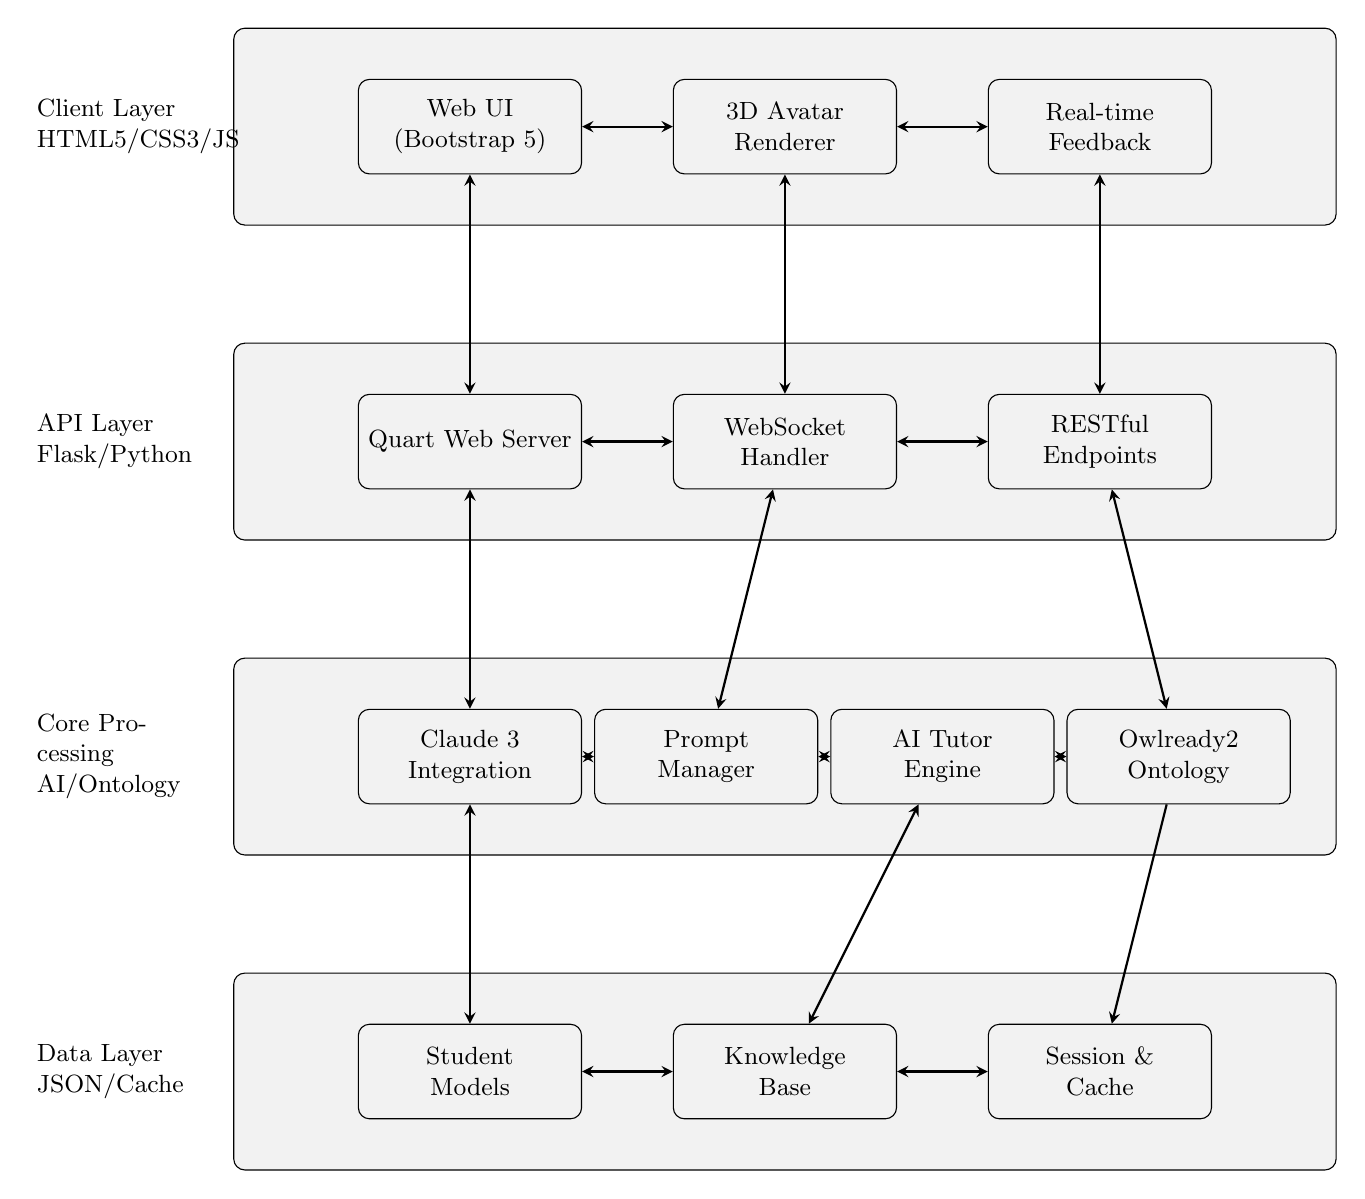
\begin{tikzpicture}[
    % Define styles for different node types
    box/.style={
        draw,
        rectangle,
        rounded corners,
        minimum width=2.8cm,
        minimum height=1.2cm,
        text centered,
        text width=2.6cm,
        font=\small
    },
    layer/.style={
        draw,
        rectangle,
        rounded corners,
        minimum width=14cm,
        minimum height=2.5cm,
        fill=gray!10
    },
    arrow/.style={
        ->,
        >=stealth,
        thick
    },
    bidirectional/.style={
        <->,
        >=stealth,
        thick
    },
    layer_label/.style={
        text width=3cm,
        align=left,
        font=\small
    }
]

% Define the layers with proper spacing
\begin{scope}[shift={(0,0)}]
    % Layer background rectangles with adjusted spacing
    \node[layer] (client) at (0,12) {};
    \node[layer] (api) at (0,8) {};
    \node[layer] (core) at (0,4) {};
    \node[layer] (data) at (0,0) {};

    % Layer labels on the left with better spacing
    \node[layer_label] at (-8,12) {Client Layer\\HTML5/CSS3/JS};
    \node[layer_label] at (-8,8) {API Layer\\Flask/Python};
    \node[layer_label] at (-8,4) {Core Pro-\\cessing\\AI/Ontology};
    \node[layer_label] at (-8,0) {Data Layer\\JSON/Cache};

    % Client Layer Components with even spacing
    \node[box] (browser) at (-4,12) {\parbox{2.6cm}{\centering Web UI\\(Bootstrap 5)}};
    \node[box] (avatar) at (0,12) {\parbox{2.6cm}{\centering 3D Avatar\\Renderer}};
    \node[box] (frontend) at (4,12) {\parbox{2.6cm}{\centering Real-time\\Feedback}};

    % API Layer Components
    \node[box] (gateway) at (-4,8) {Quart Web Server};
    \node[box] (websocket) at (0,8) {\parbox{2.6cm}{\centering WebSocket\\Handler}};
    \node[box] (endpoints) at (4,8) {\parbox{2.6cm}{\centering RESTful\\Endpoints}};

    % Core Processing Components with adjusted spacing
    \node[box] (llm) at (-4,4) {\parbox{2.6cm}{\centering Claude 3\\Integration}};
    \node[box] (prompt) at (-1,4) {\parbox{2.6cm}{\centering Prompt\\Manager}};
    \node[box] (tutor) at (2,4) {\parbox{2.6cm}{\centering AI Tutor\\Engine}};
    \node[box] (ontology) at (5,4) {\parbox{2.6cm}{\centering Owlready2\\Ontology}};

    % Data Layer Components
    \node[box] (student) at (-4,0) {\parbox{2.6cm}{\centering Student\\Models}};
    \node[box] (knowledge) at (0,0) {\parbox{2.6cm}{\centering Knowledge\\Base}};
    \node[box] (session) at (4,0) {\parbox{2.6cm}{\centering Session \&\\Cache}};

    % Vertical Connections
    \draw[bidirectional] (browser) -- (gateway);
    \draw[bidirectional] (avatar) -- (websocket);
    \draw[bidirectional] (frontend) -- (endpoints);

    \draw[bidirectional] (gateway) -- (llm);
    \draw[bidirectional] (websocket) -- (prompt);
    \draw[bidirectional] (endpoints) -- (ontology);

    \draw[bidirectional] (llm) -- (student);
    \draw[bidirectional] (tutor) -- (knowledge);
    \draw[arrow] (ontology) -- (session);

    % Horizontal Connections
    \draw[bidirectional] (browser) -- (avatar);
    \draw[bidirectional] (avatar) -- (frontend);
    \draw[bidirectional] (gateway) -- (websocket);
    \draw[bidirectional] (websocket) -- (endpoints);
    \draw[bidirectional] (llm) -- (prompt);
    \draw[bidirectional] (prompt) -- (tutor);
    \draw[bidirectional] (tutor) -- (ontology);
    \draw[bidirectional] (student) -- (knowledge);
    \draw[bidirectional] (knowledge) -- (session);
\end{scope}
\end{tikzpicture} 
    \caption{High-level System Architecture showing the four main layers (Client, API, Core Processing, and Data) and their interconnected components. The arrows indicate data flow and component interactions within and between layers.}
    \label{fig:system-architecture}
\end{figure}

\subsection{Core Components}
\label{subsec:core-components}

The system consists of the following key components:

\begin{itemize}
    \item \textbf{Client Browser:} 
        \begin{itemize}
            \item User interface components (HTML/CSS with Bootstrap)
            \item Dynamic interaction handling (JavaScript)
            \item Avatar Renderer for 3D models and animations
            \item Real-time feedback visualization
        \end{itemize}
    
    \item \textbf{Backend Server:} 
        \begin{itemize}
            \item Quart Web Server implementation
            \item RESTful API endpoints
            \item Robust session management
            \item Asynchronous request handling
        \end{itemize}
    
    \item \textbf{Tutoring System Core:} 
        \begin{itemize}
            \item Claude Tutor component for LLM integration
            \item Prompt management and optimization
            \item Student Model for knowledge tracking
            \item Adaptive learning path generation
        \end{itemize}
    
    \item \textbf{Domain Knowledge:} 
        \begin{itemize}
            \item OWL-based Physics Ontology
            \item Comprehensive Knowledge Base
            \item Concept relationship mapping
            \item Prerequisites and dependencies
        \end{itemize}
    
    \item \textbf{Persistent Storage:} 
        \begin{itemize}
            \item JSON-based student data management
            \item In-memory session handling
            \item Efficient data retrieval mechanisms
            \item Backup and recovery systems
        \end{itemize}
\end{itemize}

\section{Data Flow Architecture}
\label{sec:data-flow}

The system implements several sophisticated data flows designed to ensure efficient information processing and delivery:

\subsection{Primary Data Flows}
\label{subsec:primary-flows}

\begin{enumerate}
    \item \textbf{User Interaction Flow:}
        \begin{itemize}
            \item Frontend interface question handling
            \item AJAX request processing
            \item Real-time response display
            \item Student model visualization updates
        \end{itemize}
    
    \item \textbf{Backend Processing Flow:}
        \begin{itemize}
            \item API request routing through Quart
            \item Session instance management
            \item Response generation and formatting
            \item Error handling and recovery
        \end{itemize}
    
    \item \textbf{Tutoring System Flow:}
        \begin{itemize}
            \item Context analysis and knowledge retrieval
            \item Student model updates
            \item Adaptive response generation
            \item Learning progress tracking
        \end{itemize}
    
    \item \textbf{Knowledge Graph Flow:}
        \begin{itemize}
            \item Structured physics knowledge delivery
            \item Learning progress monitoring
            \item Concept relationship navigation
            \item Prerequisite verification
        \end{itemize}
    
    \item \textbf{Student Model Flow:}
        \begin{itemize}
            \item Concept exposure tracking
            \item Understanding level assessment
            \item Knowledge gap identification
            \item Personalized path generation
        \end{itemize}
\end{enumerate}

\section{Technology Stack}
\label{sec:tech-stack}

The system integrates modern technologies to ensure robust performance and scalability:

\begin{itemize}
    \item \textbf{Frontend Development:}
        \begin{itemize}
            \item HTML5/CSS3 with Bootstrap 5
            \item Modern JavaScript (ES6+)
            \item Responsive design principles
            \item Progressive enhancement
        \end{itemize}
    
    \item \textbf{Backend Framework:}
        \begin{itemize}
            \item Quart async Python framework
            \item RESTful API architecture
            \item WebSocket support
            \item Efficient request handling
        \end{itemize}
    
    \item \textbf{Natural Language Processing:}
        \begin{itemize}
            \item Claude 3 API integration
            \item Anthropic client implementation
            \item Context window optimization
            \item Response quality assurance
        \end{itemize}
    
    \item \textbf{Knowledge Representation:}
        \begin{itemize}
            \item Owlready2 framework
            \item OWL/RDF technologies
            \item SPARQL query optimization
            \item Semantic reasoning capabilities
        \end{itemize}
    
    \item \textbf{Data Management:}
        \begin{itemize}
            \item JSON-based storage
            \item In-memory caching
            \item Session state management
            \item Data persistence strategies
        \end{itemize}
\end{itemize}

\section{Implementation Strategy}
\label{sec:implementation}

Our implementation follows an iterative, phase-based approach:

\subsection{Development Phases}
\label{subsec:dev-phases}

\begin{enumerate}
    \item \textbf{Phase 1: Foundation}
        \begin{itemize}
            \item Environment setup and configuration
            \item API authentication implementation
            \item Basic system prompt structure
            \item Core functionality testing
        \end{itemize}
    
    \item \textbf{Phase 2: Knowledge Integration}
        \begin{itemize}
            \item Ontology development and validation
            \item Knowledge base population
            \item Context retrieval system
            \item Semantic reasoning implementation
        \end{itemize}
    
    \item \textbf{Phase 3: Adaptive Learning}
        \begin{itemize}
            \item Student model development
            \item Progress tracking mechanisms
            \item Personalization algorithms
            \item Learning path optimization
        \end{itemize}
\end{enumerate}

\section{Quality Assurance}
\label{sec:quality}

To ensure system reliability and effectiveness:

\begin{itemize}
    \item \textbf{Testing Strategies:}
        \begin{itemize}
            \item Unit testing of components
            \item Integration testing of flows
            \item Performance benchmarking
            \item User acceptance testing
        \end{itemize}
    
    \item \textbf{Monitoring and Logging:}
        \begin{itemize}
            \item System health monitoring
            \item Error tracking and reporting
            \item Performance metrics collection
            \item Usage analytics
        \end{itemize}
\end{itemize}

\section{Evaluation Framework}
\label{sec:evaluation-framework}

Our evaluation approach encompasses:

\begin{itemize}
    \item \textbf{Performance Metrics:}
        \begin{itemize}
            \item Response accuracy assessment
            \item System latency measurement
            \item Resource utilization tracking
            \item Scalability testing
        \end{itemize}
    
    \item \textbf{Educational Impact:}
        \begin{itemize}
            \item Learning outcome measurement
            \item Student engagement analysis
            \item Knowledge retention assessment
            \item Personalization effectiveness
        \end{itemize}
\end{itemize}

This methodology provides a comprehensive framework for developing and evaluating our ontology-enhanced LLM system, ensuring alignment with our research objectives and educational goals. 